\documentclass[12pt,fleqn]{article}\usepackage{../../common}
\begin{document}
Materyel Mekaniği - 6

Alttaki gibi bir kiriş düşünelim,

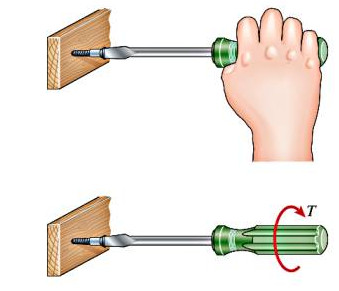
\includegraphics[width=20em]{phy_020_strs_06_01.jpg}

Daha önce bu tür bir kiriş üzerinde eksenel yöndeki kuvvetler ve yer
değişimlerinin ilişkisini

$$
\left[\begin{array}{c}
f'_{1x} \\ f'_{2x}
\end{array}\right] =
\frac{AE}{L}
\left[\begin{array}{cc}
1 & -1 \\ -1 & 1
\end{array}\right]
\left[\begin{array}{c}
u'_1 \\ u'_2
\end{array}\right]
$$

olarak göstermiştik. Üstte yazılan kirişin yerel, kendisine has kordinat
sistemini baz alıyor. Eğer üstteki değişkenleri global kordinat sistemine
eşlemek, yansıtmak istiyorsak o zaman sistemi görülen $\theta$ kadar döndürmemiz
gerekiyor. Döndürme işlemi genel olarak iki boyuttaki bir $[u, v]$ vektörü için
[1, sf. 85]

$$
\left[\begin{array}{c}
u' \\ v'
\end{array}\right] =
\left[\begin{array}{cc}
C & S \\ -S & C
\end{array}\right]
\left[\begin{array}{c}
u \\ v
\end{array}\right]
$$

ile yapılır, ki $C = \cos\theta$, $S = \sin\theta$.

Fakat unutmayalım tek eksenlikten çıktığımız zaman kirişın her ucunda iki
serbestlik derecesi vardır, her uç $u,v$ yönünde yer değişim yaşayabilir,
bunları $u_1,v_1$ ve $u_2,v_2$ diye gösterebiliriz. O zaman $u'_1,u'_2$
ile dönüş hesabı

$$
\left[\begin{array}{c}
u'_1 \\ u'_2
\end{array}\right] =
\left[\begin{array}{cccc}
C & S & 0 & 0 \\
0 & 0 & C & S
\end{array}\right]
\left[\begin{array}{c}
u_1 \\ v_1 \\ u_2 \\ v_2
\end{array}\right]
$$






[devam edecek]

Kaynaklar

[1] Logan, {\em A First Course in the Finite Element Method}

\end{document}


